\documentclass[12pt,english]{article}
%\usepackage[margin=1in,footskip=0.25in]{geometry}

%\usepackage{helvet}
%\renewcommand{\familydefault}{\sfdefault}
\renewcommand\refname{\vskip -1cm}
%\renewcommand{\rmdefault}{phv} % Arial
%\renewcommand{\sfdefault}{phv} % Arial
\usepackage{setspace}
\usepackage{wrapfig}
\usepackage{amsmath}
\usepackage{amssymb}
\usepackage{graphicx}
\usepackage{mathrsfs}
\usepackage{bm}
\usepackage{wasysym}
\usepackage{placeins}
\usepackage{multirow}
\usepackage[T1]{fontenc}
\usepackage[comma]{natbib}
\usepackage{framed}
\usepackage{caption}
\usepackage{longtable}
\usepackage{geometry}
\usepackage{lineno}

\geometry{verbose,letterpaper,tmargin=2.54cm,bmargin=2.54cm,lmargin=2.54cm,rmargin=2.54cm}


\begin{document}
\begin{spacing}{1.9}


\title{The effect of starvation on the dynamics of consumer populations}
\author{Yeakel Kempes Redner}
\maketitle

\linenumbers
%\begin{flushleft}

\section{Introduction}
%Focus on the tradeoff between REPRODUCTION AND SURVIVAL AS A FUNCTION OF ENERGETIC STATE

The behavioral ecology of most, if not all, organisms is influenced by the energetic state of individuals.
An individual's energetic state directly influences how it invests its stores in an uncertain environment.
Such behaviors are generally manifested as trade-offs, which often concern investing in individual maintenance and growth vs. producing offspring [Mangel], among a host of other behavioral duties [REFS].
The timing of these behaviors is often important and is under strong selective pressure, as they tend to have large effects on the future fitness of the organism [Mangel].
%For example, rotifers that reproduce have lower survival rates than those that don't when they are under nutritional stress.
To what extent, and when, organisms invest in these two necessary biological functions -- growth and maintenance vs. reproduction -- may be driven by habitat, seasonality, evolutionary history, inter- or intra-specific interactions, or even resource limitation.
The influence of resource limitation on an organism's ability to maintain its nutritional stores may lead to delays or shifts in reproduction. %and the subsequent loss of nutritional reserves
%Such tradeoffs are also bound to have population-level consequences, although this has received little theoretical or empirical attention.

%The reproductive vs. storage tradeoff
Maximizing fitness between growth and maintenance activities vs. reproductive behaviors in large part structures the life-history of species, and this can be achieved by a variety of potential mechanisms all of which, to some extent, depend on resource availability:
%Reproduction can be separated from somatic growth/maintenance by a variety of potential mechanisms:
%Multiple mechanisms contribute to the differentiation of these behaviors:
\emph{i}) Behavioral: The investment of time and energy towards reproductive and parental behaviors depends on resource availability \citep{Morris:1987eo}.
%, while stress can generally lead to reprodusuppression of reproductive behaviors \citep{Morgan:1999do}. 
For example, reindeer invest less in calves born after harsh winters (when the mother's energetic state is poor) than in calves born after moderate winters \citep{Tveraa:2003fq}, whereas many bird species invest differently in broods during periods of resource scarcity \citep{Daan:1988va,Jacot:2009dv}, sometimes delaying or foregoing reproduction for an entire season \citep{Barboza:2002in}.
Resource limitation can also alter the behaviors of species in well-mixed environments: freshwater and marine zooplankton have been observed to avoid reproduction under nutritional stress \citep{Threlkeld:1976ih}, while those that do reproduce evince lower survival rates \citep{Kirk:1997cc}.
Similarly, artificially induced stress has been observed to decrease reproductive success in Atlantic cod \citep{Morgan:1999do}.
\emph{ii}) Physiological: Diverse mammals (47 species in 10 families) exhibit delayed implantation whereby females postpone fetal development (blastocyst implantation), often timing with accumulation of nutritional reserves \citep{Mead:1989dt,Sandell:1990kw}. %, including multiple species of Grizzly bears (\emph{Ursus horribilis}) and the European badger (\emph{Meles melesc}) \citep{Woodroffe:1995id
Furthermore, many mammals (including humans) suffer irregular menstrual cycling and higher rates of spontaneous abortion during periods of nutritional stress \citep{Bulik:1999eo,Trites:2003cc}.
\emph{iii}) Spatio-temporal: Organisms may also separate maintenance/growth from reproduction over space and time. 
For example, many salmonids, birds, and some mammals return to migratory breeding sites to reproduce after one or multiple seasons in alternative environments spent accumulating body mass and nutritional reserves \citep{Weber:1998jg,Mduma:1999cp,Moore:2014hi}.
%great tits invest more energy into broods when resource abundance is greater, while food availability is generally seen to correlate with clutch size among many bird species \citep{Daan:1988va}.
%The mechanisms that control reproductive effort as a function of energetic reserves differ among species.
%Even humans alter their growth trajectories and have higher chances of fetal abortion during periods of starvation.
%Thus, some organisms partition reproductive vs. foraging effort over both space and time, whereas other rely on physiological mechanisms to optimize reproductive success against survival when adequate resources are unavailable.
The existence of so many independently evolved mechanisms across such a diverse suite of organisms points to the importance and universality of the fundamental tradeoff between spending energy on ones own tissues and spending energy on passing down genetic material.

%To population-level effects
Organisms employ different strategies to avoid reproduction during times of nutritional stress, and how this is achieved has received tremendous empirical and theoretical attention, owing to the importance of these activities in shaping life-history [REF].
Less well understood is how resource limitation affect dynamics at the level of the population when organisms are able to avoid the risk of spending energy on reproduction when starvation is likely.
Traditional Lotka-Volterra models assume a dependence of consumer population growth rates on resource density, thus implicitly incorporating the requirement of resource availability for reproduction.
However, resource limitation and the subsequent effects of starvation can also be accounted for \emph{explicitly}, such that reproductive growth of a population is only allowed to occur if individuals have sufficient energetic reserves.
Incorporating energetic dynamics that occur on an individual level [REF] into a population-based framework \citep{Kooi2000,Sousa:2010ez}, though straightforward conceptually, has many challenges that arise mathematically \citep{Diekmann:2010da}, and this has limited simple theoretical models aiding our understanding of larger-scale dynamics.

%What we did...
Here we explore how reproductive trade-offs, which occur at the level of the individual, may influence the dynamics of a population.
We first establish a simple stage-structured population model that captures the essential dynamics of energetic reproductive tradeoffs, and explore the impact of different fluxes on system-level stability.
By relating different rate constants to allometric relationships, we uncover important constraints in the timescales of different physiological processes that determine dynamics and investigate how organisms of alternative body sizes and taxonomic affinities are expected to evince contrasting population-level dynamics.
We then develop a more general dynamic model in order to understand if there are common attributes of these energetically-constrained systems that have implications beyond assumptions inherent to the specific model.
We show [WHAT]?
%Finally, we compare our population-dynamic approach with a stochastic dynamic program that incorporates different individual-level behaviors as a function of energetic state.


%We devise the simplest energetic-compartment system to investigate the effects of a reproductive tradeoff with starvation on population dynamics.

%FITNESS and ENERGETICS... the model incorporates fitness consequences of energetic loss... 

\section{Methods}
\subsection{Model description}

We first integrate energetics into the dynamics of a consumer-resource system by assuming that the consumer population can be divided into discrete energetic states, the occupation of each being contingent on the consumption of a single resource $R$.
In the simplest case, there are only two energetic states for the consumer population: \emph{i}) an energetically replete (full) state $F$, where the consumer reproduces at rate $\lambda$, and \emph{ii}) an energetically deficient (hungry) state $H$, where reproduction is suppressed, and mortality occurs at rate $\mu$.
Consumers transition from state $F$ to state $H$ by starvation at rate $\sigma$ and in proportion to the lack of food $1-R$.
Conversely, consumers recover from state $H$ to the full state $F$ at rate $\rho$ and in proportion to the density of resources consumed $R$.
The resource has logistic growth with a linear growth rate $a$ and a carrying capacity of unity.
Resources are eliminated by the consumer in either state: by energetically deficient consumers at rate $\rho$, and by energetically replete consumers at rate $b$.
Accordingly, the system of equations is written

\begin{align}
\frac{\rm d}{\rm dt} F &= \lambda F + \rho HR - \sigma (1-R)F, \nonumber \\
\frac{\rm d}{\rm dt} H &= \sigma (1-R)F - \rho RH - \mu H, \nonumber \\
\frac{\rm d}{\rm dt} R &= a R(1-R) - R(\rho H+ b F).
\label{eq_specific}
\end{align}

There are three steady states for the 2-stage consumer-resource system: two trivial steady states at $(R^*=0,H^*=0,F^*=0)$ and $(R^*=1,H^*=0,F^*=0)$, and one non-trivial internal steady state where $(R^*>0,H^*>0,F^*>0)$.
The latter steady state is the one of chief ecological interest, where

\begin{align}
F^* &= \frac{a  \lambda  \mu  (\mu +\rho )}{(\lambda  \rho +\mu  \sigma ) (\lambda  \rho +\mu  m)}, \nonumber \\
H^* &= \frac{a  \lambda ^2 (\mu +\rho )}{(\lambda  \rho +\mu  \sigma ) (\lambda  \rho +\mu  m)}, \nonumber \\
R^* &= \frac{\mu  (\sigma -\lambda )}{\lambda  \rho +\mu  \sigma }.
\end{align}

\noindent Because there is only one internal steady state, as long as it is stable the population trajectories will be globally attracted to it for any set of initial conditions greater than zero.

Analysis of the stability of the consumer-resource system is explored with respect to the local stability of the internal steady state, which is the only feasible steady state as long as both the consumer and resource have non-zero, positive, values.
In a multidimensional system, linear stability is determined with respect to the Jacobian Matrix $\bf J$, which is a matrix where each element is defined by the partial derivative of each equation with respect to each variable.
In the case of the 2-stage consumer model, the Jacobian evaluated at the internal steady state (denoted by $|_*$) is written

\begin{equation}
\mathbf{J}|_* =
%\left(
%\begin{array}{ccc}
% -F^* m+(1-R^*) a -R^* a -H^* \rho  & -R^* \rho  & -m R^* \\
% -H^* \rho -F^* \sigma  & -\mu -R^* \rho  & (1-R^*) \sigma  \\
% H^* \rho +F^* \sigma  & R^* \rho  & \lambda -(1-R^*) \sigma  \\
%\end{array}
%\right).
\left(
\begin{array}{ccc}
 -\frac{\lambda  \rho  (\sigma - \lambda )}{\lambda  \rho +\mu  \sigma } & \frac{\mu  \rho  (\sigma -\lambda )}{\lambda  \rho +\mu  \sigma } & \frac{\alpha  \lambda  (\mu +\rho )}{m \mu +\lambda  \rho } \\
 \frac{\lambda  (\mu +\rho ) \sigma }{\lambda  \rho +\mu  \sigma } & -\frac{\mu  (\mu +\rho ) \sigma }{\lambda  \rho +\mu  \sigma } & -\frac{\alpha  \lambda  (\mu +\rho )}{m \mu +\lambda  \rho } \\
 -\frac{m \mu  (\sigma - \lambda)}{\lambda  \rho +\mu  \sigma } & -\frac{\mu  \rho  (\sigma - \lambda )}{\lambda  \rho +\mu  \sigma } & -\frac{\alpha  \mu  (\sigma - \lambda)}{\lambda  \rho +\mu  \sigma } \\
\end{array}
\right).
\end{equation}


%Transcritical bifurcation
If the parameters of the Jacobian matrix at the internal steady state are such that its leading eigenvalue is $<0$, then the system is stable to small pulse perturbations, conditioned on the value of the starvation rate $\sigma$ relative to the value of the consumer reproduction rate $\lambda$.
As $\sigma$ nears and becomes lower than a given $\lambda$, the resource steady state $R^*$ crosses the origin and exchanges stability to become unstable.
As such, a transcritical bifurcation exists at $\lambda = \sigma$, such that the existence of an internal stable fixed point is dependent on the condition that $\sigma > \lambda$.
Biologically, this means that the rate of starvation is greater (operating on a smaller timescale) than the rate of consumer reproduction (operating on a relatively longer timescale).
As will be shown in Section XX, this general expectation will hold for most classes of organisms, while the exact difference in timescales between reproduction and starvation can be derived using allometric scaling relationships.
%Kempes (REF) has shown that population growth rates scale to $M^{\alpha-1}$ (where $M$ is the reproductive mass of an organism and $\alpha$ is the scaling exponent), whereas starvation is necessarily bound to shorter timescales, which will be elaborated on below.


%Hopf bifurcation
Oscillating, or cyclic, dynamics present additional risks to populations.
If cycles are large, stochastic effects may result in extinction.
In continuous-time systems, cycles arise when a pair of complex conjugate eigenvalues cross the imaginary axis and attain positive real parts.
%Of additional interest is the existence of parameter regions that permit the existence of oscillatory, or cyclic, dynamics.
This condition is called a Hopf bifurcation, and is defined by ${\rm Det}({\bf S}) = 0$, where $\bf S$ is the Sylvester matrix, which is composed of the coefficients of the characteristic polynomial describing the Jacobian matrix.
Although the Hopf condition for the specific 2-stage model cannot be easily written, the analytical solution can be explored using a symbolic computational language such as \emph{Mathematica}.


\subsection{Analysis of a generalized model}

We may gain additional insight by that we do not know the specific rate functions from our 2-stage consumer resource model presented in Eq. \ref{eq_specific}.
For example, we assume a linear mortality term for hungry foragers $\mu H$, though we may wish to assert that our knowledge of consumer mortality involves those that are energetically deficient, but nothing else.
In this case, we would assume only that the rate of mortality is governed by the function $M(H)$.
Substituting general functions for all rate laws from Eq. \ref{eq_specific}, we obtain the generalized ODE system

\begin{align}
\frac{\rm d}{\rm dt} F &= G(F) + S(R,H) - K(R,F), \nonumber \\
\frac{\rm d}{\rm dt} H &= K(R,F) - S(R,H) - M(H), \nonumber \\
\frac{\rm d}{\rm dt} R &= P(R) - L(R,H,F).
\label{eq_gen}
\end{align}

\noindent where $G(F)$ determines consumer growth, $S(R,H)$ and $K(R,F)$ are the recovery and starvation functions, respectively, $M(H)$ determines consumer mortality, and $P(R)$ and $L(R,H,F)$ are functions describing the growth and consumption-loss of resources, respectively.


If the system is written in this generalized manner, we cannot solve for the steady state solution $(F^*,~H^*,~R^*)$, however we can normalize the system to the unknown steady states.
We denote normalized variables and functions in lowercase, such that $f = F/F^*$, $h = H/H^*$, $r = R/R^*$, and for example the normalized mortality function $m(h) = M(H)/M^*$, where $M^*$ is shorthand for $M(H^*)$.
Additional rearrangements of terms under equilibrium conditions allows us to define two additional sets of scaling parameters with intuitive biological properties: the turnover rates of full foragers, hungry foragers, and the resource ($\alpha_f$, $\alpha_h$, $\alpha_r)$, and the proportional branching biomass through different compartments of the model, generally designated by the parameter $\beta$.
For instance, $\beta_f$ is the proportion of full consumer growth due to reproduction, whereas $(1-\beta_f)$ is the proportion of full consumer growth due to recruitment \emph{from} the hungry forager class.
Similarly, $\beta_h$ is the proportion of hungry consumer loss due to mortality, whereas $(1-\beta_h)$ is the proportion of hungry consumer loss due to recruitment \emph{into} the full consumer class (see SUPP for a detailed derivation).
Substituting the normalized variables and functions into Eq. \ref{eq_gen}, we obtain

 
\begin{align}
\dot{f} &= \alpha_f \left[ \beta_f g(f) + (1-\beta_f)s(r,h) - k(r,f)\right], \nonumber \\
\dot{h} &= \alpha_h \left[ k(r,f) - (1-\beta_h)s(r,h) - \beta_h m(h) \right], \nonumber \\
\dot{r} &= \alpha_r \left[ p(r) - l(r,h,f) \right],
\label{eq_gen}
\end{align}

\noindent and linearization of this normalized, general ODE system yields the Jacobian matrix

\begin{equation}
\mathbf{J}_{\rm gen}|_* =
\left(
\begin{array}{ccc}
 \alpha_f \left(\beta_f \frac{\partial g}{\partial f} - \frac{\partial k}{\partial f} \right) & \alpha_f(1-\beta_f)\frac{\partial s}{\partial h} & \alpha_f \left( (1-\beta_f)\frac{\partial s}{\partial r} - \frac{\partial k}{\partial r} \right) \\
 \alpha_h \frac{\partial k}{\partial f} & -\alpha_h \left(\beta_h \frac{\partial m}{\partial h} + (1-\beta_h) \frac{\partial s}{\partial h} \right) & \alpha_h \left(\frac{\partial k}{\partial r} - (1 - \beta_h)\frac{\partial s}{\partial r} \right) \\
 -\alpha_r \frac{\partial l}{\partial f} & -\alpha_r \frac{\partial l}{\partial h} & \alpha_r \left( \frac{\partial p}{\partial r} - \frac{\partial l}{\partial r} \right) \\
\end{array}
\right).
\label{eq_Jacgen}
\end{equation}

%Importance of the elasticities
Due to the normalization procedure, the partial derivatives in Eq. \ref{eq_Jacgen} have tangible biological meaning.
Because, for example, the partial derivative (containing functions and variables normalized to the unknown steady states) $\partial g / \partial f = \partial \log G / \partial \log F$, it scales in such a way that it represents the percent change in consumer growth (governed by $G(F)$) relative to a percent change in the density of full consumers $F$, more commonly known as a functional elasticity.
For example, if growth is a linear function (e.g. $G(F) = \lambda F$), $\partial g / \partial f = 1$; if growth is a quadratic function (e.g. $G(F) = \lambda F^2$), $\partial g / \partial f = 2$, while more complex functions may depend on the value of the steady state.
For example, if consumer growth is modeled as Holling Type II growth, such that $G(F) = c_1 F^2/(c_2 + F^2)$, where $c_1$ and $c_2$ are unknown constants, then its elasticity will vary between $0$ and $2$, depending on the steady state value $F^*$, which is unknown in the generalized system.

%Why do this?
%The normalization of the generalized system described above results in the inclusion of functional elasticities into the generalized Jacobian matrix. 
Deriving a Jacobian in terms of the normalized ODE system is useful because it allows us to place strict constraints on the values of the unknown variables (the turnover rates, biomass branching parameters, and the functional elasticities), without assuming detailed knowledge of the functions controlling different rates within the system. % retaining the fundamental architecture of the 2-class consumer-resource system.
%Simplifications
In addition, we can now insert a number of assumptions that will align our generalized Jacobian more closely with the original 2-stage consumer resource system.
We will assume the following:
\emph{i}) both the consumer and resource suffers linear mortality,
\emph{ii}) resource growth is logistic,
\emph{iii}) recovery and starvation are linear with respect to both full and hungry consumer densities, and
\emph{iv}) consumers and resources have equivalent turnover rates scaled to unity.
These assumptions lead to the following simplifications

\begin{align}
	i)~&\frac{\partial m}{\partial h} = 1, ~~~~~~~~ \frac{\partial l}{\partial r} = 1, ~~~~~~~~ \frac{\partial l}{\partial f} = 1 - \frac{\partial l}{\partial h}, \nonumber \\
	ii)~&\frac{\partial k}{\partial r} = \left(1 - \frac{1}{R^*} \right)^{-1}, \nonumber \\
	iii)~&\frac{\partial s}{\partial r} = \frac{\partial s}{\partial h} = 1, ~ \frac{\partial k}{\partial f} = 1, \nonumber \\
	iv)~&\alpha_f = \alpha_r = 1,
\end{align}

\noindent where $R^*$ ranges from 0 to 1.
The remaining free parameters include the timescale of hungry foragers $\alpha_h$, the branching parameters $\beta_f$ and $\beta_h$, the elasticity of consumer growth with respect to full consumer densities $\partial g / \partial f$, the elasticity of resource growth with respect to resource density $\partial p / \partial r$, the elasticity of resource loss with respect to full consumer density $\partial l / \partial f$, and the elasticity of starvation with respect to resource density $\partial k / \partial r$.
See Table XX for a list of the free parameters in the generalized model, as well as the ranges of potential values for each.
These substitutions result in the simplified Jacobian matrix

\begin{equation}
\mathbf{J}_{\rm gen}|_* =
\left(
\begin{array}{ccc}
 \left(\beta_f \frac{\partial g}{\partial f} - 1 \right) & (1-\beta_f) & \left( (1-\beta_f)\frac{\partial s}{\partial r} - 1 \right) \\
 \alpha_h & -\alpha_h & -\alpha_h \left(1-\frac{\partial k}{\partial r} - \beta_h  \right) \\
 \frac{\partial l}{\partial h}-1 & -\frac{\partial l}{\partial h} &  \left( \frac{\partial p}{\partial r} - 1 \right) \\
\end{array}
\right).
\label{eq_Jacgen}
\end{equation}

%Testing stability
Because the remaining free parameters have known ranges, but not specific values, we wish to assess the correlations of each to system stability.
By randomly drawing values from uniform distributions bounded by the known ranges of each free parameter, we obtain an ensemble of potential Jacobian matrices whereupon the stability of each is determined by numerically calculating the real part of the leading eigenvalue.
If the real part of the leading eigenvalue is $<1\times10^{-6}$, we assumed the system to be stable.
Replicating this procedure on the order of $10^7$ times allowed us to determine the correlation of each free parameter with stability to the extent that variance was negligible.



\subsection{Allometric scaling relationships}

Nearly all of the rates described in the specific model, and generalized upon in the generalized model, are to some extent governed by the body size of the consumer.
The scaling relationship between an organism's metabolic rate $B$ and its body size at reproductive maturity $M$ plays a central role in other scaling relationships.
Organismal metabolic rate $B$ is known to scale as $B = B_0 M^\eta$, where $\eta$ is the scaling exponent, generally assumed to be 3/4 for metazoans, etc.
Kempes et al. [REF] show how the population-level growth rate also can be related to body size as $\lambda = \lambda_0 M^{\eta-1}$.

Population growth requires that individuals 


%\begin{align}
%\lamdba &=  \nonumber \\
%\sigma &= \nonumber \\	
%\end{align}


\section{Results}

\subsection{2-stage consumer resource model}

Analysis of the continuous-time 2-stage consumer resource model shows that the equilibrial states of both populations are highly sensitive to changes in  starvation and recovery rates of the consumer.
The consumer and resource population densities vary inveresely: when the consumer densities are high, resource densities are low, and vice versa.
High starvation and low recovery rates result in low consumer densities and high resource densities. %whereas the opposite is true for low starvation and high recovery rates.
If starvation rates are low, resources have a fixed point near zero for any value of the recovery rate.
Full and hungry consumer stages tend have fixed points that are tightly correlated, the extent to which is driven by the similarity of consumer growth and mortality rates; if $\lambda = \mu$, then $F^* = H^*$.

%Transcritical & rate law ranges
A transcritical bifurcation exists at $\lambda = \sigma$, such that the condition $\sigma > \lambda$ is required for biologically reasonable dynamics.
The TC bifurcation occurs in this model because we have assumed that all energetically replete individuals reproduce at the same rate, whereas the traditional Lotka-Volterra dynamic assumes that the reproductive rate of the consumer is scaled to resource density, such that the growth function would be $G(F,R) = \lambda R F$.
Thus, the Lotka-Volterra dynamic \emph{implicitly} accounts for starvation in reducing the reproductive rate of the consumer.
However, our 2-stage model \emph{explicitly} accounts for starvation as well as recovery, such that individuals who are not starved should adopt a reproductive rate independent of resource density.

The existence of the transcritical bifurcation reveals important biological insight.
Reproduction requires maintenance and growth of biological tissues, both of which have strong scaling relationships with body size.
Recent work by Kempes et al. [REF] derived the timescale of reproduction in terms of allometric considerations, where $t_\lambda \propto M^{1-\eta}$ (REF).
Starvation is the loss of energy required for maintenance, and we have shown it to have a timescale $t_\sigma \propto \log(M)$.
Accordingly, the timescale of reproduction is always larger than the timescale of starvation, such that $\lambda < \sigma$.
A third important parameter in our framework is the rate of recovery.
The recovery timescale $t_\rho$ controls the rate at which individuals move from the hungry class to the full class, and this requires not only tissue maintenance, but growth, such that it is bounded on the short side by $t_\sigma$.
Moreover, [why is recovery timescale bounded on the high side], such that it is bounded on the long side by $t_\lambda$.

We have used scaling relationships between tissue turnover and growth to strictly constrain 5/6 population-level parameters in our 2-stage consumer resource model (including the mortality rate $t_\mu$, which we have shown is just a xxx of $t_\sigma$).
This exercise accomplishes two goals:
1) it allows us to constrain the plausible parameter space of the two-stage model, and 
2) 

This allows us to derive many aspects of the system in terms of consumer body mass $M$ and the allometric scaling exponent $\eta$.



\subsection{Generalized analysis}
Constraining the model with allometric scaling relationships yields important insights regarding the tradeoff between [fitness and energy]


%The natural ordering of the scaled rates
%lambda < rho < sigma
%if lambda is 0.2, and sigma is 0.8, then rho is between 0.2 and 0.8.
%In other words, lambda has the SLOWEST timescale, sigma has the fastest timescale, and rho has a timescale intermediate to both.



\section{Discussion}

%The reproductive tradeoff as a strategy
%
% \begin{figure}[h]
% 	\centering
% 	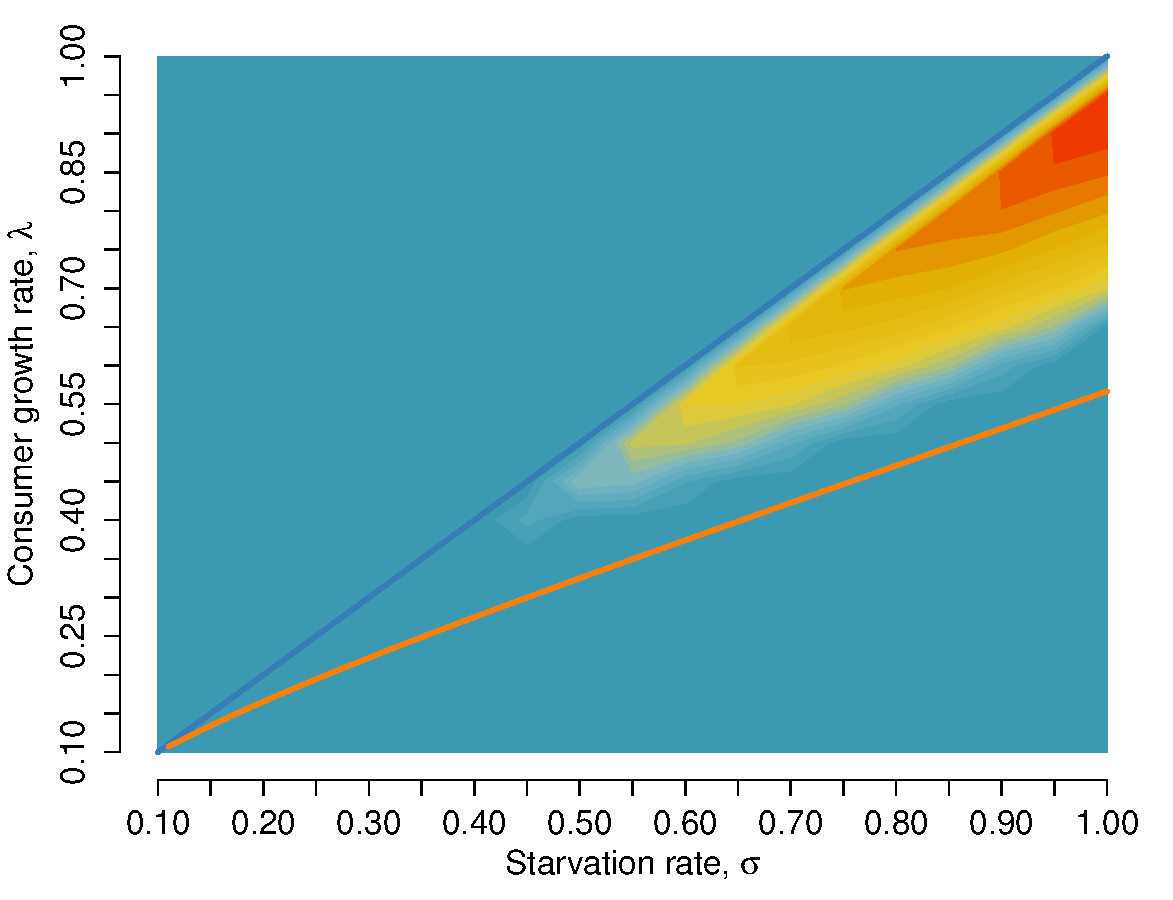
\includegraphics[width=0.5\textwidth]{fig_Hopf.pdf}
% 	\caption{
% 	Saddle Node bifurcation
% 	}
% 	\label{SN}
% \end{figure}
%
%
% \begin{figure}[h]
% 	\centering
% 	\includegraphics[width=0.5\textwidth]{fig_resvuln.pdf}
% 	\caption{
% 	Probability that the resource value is less than threshold = 0.05
% 	}
% 	\label{SN}
% \end{figure}
%
%
%
% \begin{figure}[h]
% 	\centering
% 	\includegraphics[width=0.5\textwidth]{fig_Competition.pdf}
% 	\caption{
% 	Hopf bifurcation
% 	}
% 	\label{SN}
% \end{figure}


\bibliographystyle{ieeetr} % for Science,
\bibliography{aa_starving}

%\end{flushleft}
\end{spacing}
\end{document}
